%Alle Daten sind auf dem Stand vom 22.08.12 (bei den Links steht der Tag des Aufrufs dahinter)
\begin{multicols}{2}[\subsection{Alle wichtigen Anlaufstationen und Adressen}]

Wir zeigen euch hier (ohne Garantie auf Vollständigkeit) eine Liste der  wichtigsten Ansprechpartner und Institutionen. Am besten schaut ihr aber selber im Internet nach und sucht euch den aktuellen Verantwortlichen heraus. Die wichtigsten Internetadressen dafür sind:

\begin{itemize}\itemsep 0pt
    \item Fachbereich Mathematik:\\
		\url{http://www.math.uni-hamburg.de} %Stand: 22.08.12
    \item Studienbüro des Fachbereichs Mathematik:\\          
    	\url{http://www.math.uni-hamburg.de/studienbuero/} %Stand: 22.08.12
    \item Beauftragte am Fachbereichs Mathematik:\\          	
    	\url{http://www.math.uni-hamburg.de/contact/beauftragte.html} %Stand: 22.08.12
    \item Alle Mitarbeiter des Fachbereichs Mathematik:\\          
    	\url{http://www.math.uni-hamburg.de/contact/mitarbeiter.html} %Stand: 22.08.12
    \item Fachbereich Wirtschaftswissenschaften:\\     
    	\url{http://www.wiso.uni-hamburg.de} %Stand: 22.08.12
    \item TU Harburg:\\
    	\url{http://www.tuhh.de} %Stand: 22.08.12
    \item Service für Studierende:\\          
    	\url{http://www.verwaltung.uni-hamburg.de/vp-1/3/33/index.html} %Stand: 22.08.12
    \item Zentrale Studienberatung und Psychologische Beratung:\\
    	\url{http://www.verwaltung.uni-hamburg.de/campuscenter/ueber-uns/studienberatung-und-psychologische-beratung/index.html} %Stand: 22.08.12
\end{itemize}
Für die verschiedenen Studiengänge sind Mailinglisten eingerichtet. Alle relevanten Informationen werden per E-Mail an alle eingetragenen Adressen verschickt. Jeder sollte sich daher unbedingt in seine Mailingliste eintragen.Dieses könnt ihr auf der entsprechenden, folgenden Seite machen.

\begin{center}
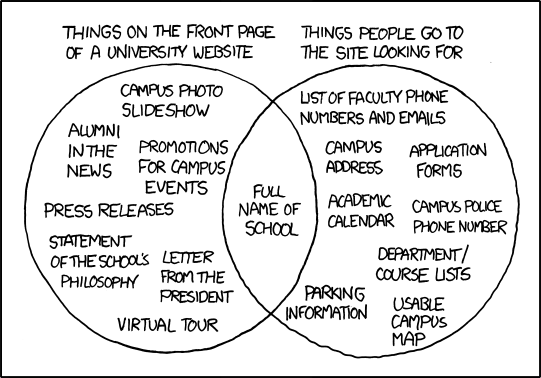
\includegraphics[scale=.65]{comics/733}
\end{center}

\begin{itemize}\itemsep 0pt
\item Bachelor Mathematik\\          	
	\url{https://mailman.rrz.uni-hamburg.de/mailman/listinfo/bama} %Stand: 22.08.12
\item Bachelor Wirtschaftsmathematik\\          
	\url{https://mailman.rrz.uni-hamburg.de/mailman/listinfo/bawima} %Stand: 22.08.12
\item Lehramt an Gymnasien und Berufliche Schulen\\          
	\url{https://mailman.rrz.uni-hamburg.de/mailman/listinfo/lamagymbs} %Stand: 22.08.12
\item Lehramt an der Primar- und Sekundarstufe I, Lehramt an Sonderschulen\\
	\url{https://mailman.rrz.uni-hamburg.de/mailman/listinfo/lamapss} %Stand: 22.08.12
\end{itemize}
Wenn ihr euch mit Professoren oder anderen Mitarbeitern treffen wollt, ist es häufig sinnvoll, den Kontakt zunächst per E-Mail herzustellen und dann einen Termin abzusprechen. Wegen kleinerer Angelegenheiten kann man die meisten Professoren bei deren Anwesenheit häufig auch außerhalb der Sprechstunden aufsuchen.
\end{multicols}

\subsubsection{Studienfachberatung}

%% Informationen sind online unter
%% http://www.math.uni-hamburg.de/teaching/service/studienfachberatung.html
%% zu finden.

\begin{tabularx}{\textwidth}{|X|X|X|X|}
\hline Bachelor Mathematik&Studienbüro Mathematik&Di, Mi, Do \hfill 10-12
	&Räume E14, E16, E18\\
	&studienbuero@math.uni-hamburg.de&Di, Mi \hfill13-15&\\
\hline Bachelor Wirtschaftsmathematik %&Prof. Dr. Hans Daduna& \hfill    &Raum T17 \\
%&hans.daduna@math.uni-hamburg.de&&+49 40 42838-4930\\
%&&&\\
&Prof. Dr. Natalie Neumeyer& \hfill &Raum T13\\
&natalie.neumeyer@math.uni-hamburg.de&&+49 40 42838-4907\\
\hline Bachelor Lehramtsstudiengänge&&&\\
Lehramt Gymnasium und Berufliche Schulen&Prof. Dr. Ingo Runkel&&Raum 309\\
    &ingo.runkel@math.uni-hamburg.de&&+49 40 42838-5172\\
    &&&\\
Lehramt Primar- und Sekundarstufe I, Lehramt an Sonderschulen
    &Prof. Dr. Andrea Blunck& \hfill &Raum 211\\
    &andrea.blunck@math.uni-hamburg.de&&+49 40 42838-5160\\
    &&&\\
\hline Master Mathematik
    &\multicolumn{3}{|l|}{Studienbüro Mathematik, siehe Bachelor Mathematik}\\
\hline
\end{tabularx}

\subsubsection{Spezielle Fragen Lehrerprüfungsamt zu den Lehramtsprüfungen für Lehramtsstudierende mit Abschlussziel 1. Staatsexamen
}

\begin{tabularx}{\textwidth}{|X|X|X|X|}
\hline Lehrerprüfungsamt&Mümmelmannsberg 75&Mo, Do \hfill 9-12
    &+49 040 42854-7611\\
    &&Di \hfill 14-15:30&\\
\hline
\end{tabularx}

\subsubsection{Spezielle fachübergreifende Fragen zur Prüfungsverwaltung für Lehramtsstudierende mit Abschlussziel BA/MA}

\begin{tabularx}{\textwidth}{|X|X|X|X|}
\hline Zentrales Prüfungsamt für die Lehramtsprüfungen der Universität Hamburg (ZPLA)&Bogenallee 11, 2. OG.&Mo-Do \hfill 10-13
    &+49 040 42838-7529\\
\hline
\end{tabularx}


\subsubsection{BAföG-Vertrauensdozenten}

\begin{tabularx}{\textwidth}{|X|X|X|}
\hline Prof. Dr. Hans Joachim Oberle&Di,Fr \hfill 9-10&Raum 120\\
       oberle@math.uni-hamburg.de&&+49 40 42838-5113\\
\hline Prof. Dr. Thomas Andreae&Di, Fr \hfill 14-14:30&Raum 238\\
       andreae@math.uni-hamburg.de&&+49 40 42838-5196\\
\hline
\end{tabularx}

\subsubsection{Beauftragter für ausländische Studierende}
\begin{tabularx}{\textwidth}{|X|X|X|}
\hline Prof. Dr. Ingenuin Gasser& \hfill &Raum 105\\
       ingenuin.gasser@math.uni-hamburg.de&&+49 40 42838-5128\\
\hline
\end{tabularx}

\subsubsection{Fachschaftsrat Mathematik}

\begin{tabularx}{\textwidth}{|X|X|X|}
\hline Fachschaftsrat Mathematik&&Raum T30\\
       fsr@math.uni-hamburg.de&&\\
\hline
\end{tabularx}

\subsubsection{Wichtige Adressen und Telefonnummern}

\begin{tabularx}{\textwidth}{|X|X|X|X|}
\hline FSR Wirtschaftswissenschaften&Von-Melle-Park 5&Raum 0070&+49 40 441266\\
       \url{http://wiwifsr.de/}&&&\\ %Stand: 22.08.12
\hline FSR Physik&Jungiusstraße 9&Raum 020&+49 40 352 202\\
       \url{http://fsrix.physnet.uni-hamburg.de/}&&&\\ %Stand: 22.08.12
\hline FSR Informatik&Vogt-Kölln-Str. 30&Sitzungen: C-101&+49 40 5404228\\
       \url{http://www.informatik.uni-hamburg.de/Fachschaft/wiki/index.php/Fachschaftsrat}&&&\\ %Stand: 22.08.12
\hline FSR Elektrotechnik&Schwarzenbergstraße 95&Raum E 0.098&+49 40 42878-2975\\
       \url{http://fsr-etit.de/}&&&\\ %Stand: 22.08.12
\hline FSR Maschinenbau&Schwarzenbergstraße 95&Raum 0.101&+49 40 42878-4008\\
       \url{http://cgi.tu-harburg.de/~fsrmwww/doku.php?id=start}&&&\\ %Stand: 22.08.12
\hline Studierendenwerk Hamburg&Von-Melle-Park 2&&+49 40 41902-0\\
       \url{http://www.studierendenwerk-hamburg.de}&&&\\ %Stand: 22.08.12
\hline
\end{tabularx}
\clearpage
